\chapter{Introduction to Power}
What is Power Electronics?

\begin{pline}
    \item \textbf{Source:} something that generates power
    \item \textbf{Load:} something that consumes power
    \item \textbf{Power electronics:} application of electronics and circuitry to control the conversion of one form to another
\end{pline}

Converter types between AC and DC Power: DC stands for "direct current" and can be visualized as a constant voltage over time. One example is a battery and photovoltaic panel. AC power stands for "alternating current" and is a sinusoidal voltage in time. An example of this is the power from the outlet. There are four basic types of converters.
\begin{pline}
    \item AC-DC: AC source to DC load, which is commonly called a rectifier like in the use of a laptop charger
    \item DC-DC: DC source to DC load, battery pack USB
    \item DC-AC: DC source to AC load, also commonly called an inverter like for a photovoltaic to grid system
    \item AC-AC: AC source to AC load, not as common but used in wond power system
\end{pline}

\section{Average and Root Mean Square (RMS) Calculations}
Period waveforms repeat their shape across each period. The average value of a sine wave is 0. $\langle v(t) \rangle = \frac{1}{T} \int_0^T v(t) \,dt$ will represent the average value here.

The RMS is represented as capital V listed below
\begin{define}
    \[V = \sqrt{\frac{1}{T} \int_0^T v(t)^2 \,dt}\]
\end{define}
We can think of the RMS value as the equivalent voltage if we put the waveform of choice across a resistor

The power is equal to the voltage waveform squared over the resistor. The triangle brackets represent the average here.
\begin{define}
    \[\langle P \rangle = \langle \frac{v^2}{R} \rangle = v^2\]
\end{define}
Remember that 
\[\langle v \rangle ^2 \neq v^2\]

If we take a look at this sine wave and say that this represents current and connected this to a resistor, average power would not be 0 even though average current is 0. $I(t)$ here represents the instantaneous value. The resistor generates (consumes) power at both the negative and positive parts of this waveform.

\begin{figure}[H]
    \centering
    \begin{tikzpicture}
        % Axes
        \draw[->] (0,0) -- (6.5,0) node[right] {$t$};
        \draw[->] (0,-1.5) -- (0,1.5) node[above] {$I(t)$};
        
        % Sine wave
        \draw[domain=0:2*pi,smooth,variable=\x,blue] plot ({\x},{sin(\x r)});
        
        % Labeling
        \draw[dashed] (pi/2,0) -- (pi/2,1) node[pos=0.5, right] {$\frac{\pi}{2}$};
        \draw[dashed] (3*pi/2,0) -- (3*pi/2,-1) node[pos=0.5, left] {$\frac{3\pi}{2}$};
        
        % Axes labels
        \node[below] at (pi,0) {$\pi$};
        \node[below] at (2*pi,0) {$2\pi$};
        \node[left] at (0,1) {1};
        \node[left] at (0,-1) {-1};
    \end{tikzpicture}
\end{figure}

\begin{sanity}
    Is the RMS value always greater than or equal to the average value? Yes. Recall the definitions of average value and the RMS value above. My intuition behind this is that you're squaring a periodic function there will be no negative values.
\end{sanity}

Sine wave RMS value calculations:

Define $x(t) = X_{peak} \sin{(t \times \frac{2\pi}{T})}$. We multiply $t$ by a factor of $\frac{2\pi}{T}$ since we are working in units of time.
\begin{align*} 
    X_{RMS} &= \sqrt{\frac{1}{T} \int_0^T X_{peak}^2 \sin^2{(t \times \frac{2\pi}{T})} \,dt} \tag{1} \\
    &= \sqrt{\frac{X_{peak}^2}{T} \int_0^T (1-\cos{(2\cdot \frac{2\pi}{T})}) \,dt} \tag{2} \\
    &= \sqrt{\frac{X_{peak}^2}{2T} \left[t \mid_0^T - \sin{(\frac{4\pi t}{T})\frac{T}{4\pi} \mid_0^T}\right]_0^T} \tag{3} \\ 
    &= \sqrt{\frac{X_{peak}^2}{2T} \left[T - \frac{T}{4\pi}(\sin{(4\pi) - \sin{(0))}}\right]_0^T} \tag{4} \\
    &= \frac{X_{peak}}{\sqrt{2}} \tag{5}
\end{align*}

Line (2) comes from the trig idenity 
    \[\sin^2{u} = \frac{1-\cos{(2u)}}{2}\]
Line (3) comes from evaluating the integral. In line (4), we see that everything within the brackets evaluates to $T$ and that this results in $T$ cancelling out with the $T$ in the denominator, resulting in just a 2 in the denominator, which is later square rooted.

\section{Oscilloscope Readings}
We notice that $X_{peak}$ is described in its RMS value as the large value that we can get. The amplitude of this sine wave is 1, but if we were to output this sinusoid in High-Z mode on the function generator, we would have to set this to a 2 $V_{pp}$ (Volt peak to peak). Contrastingly, if we were in 50-Ohm mode, setting the function generator to 2 $V_{pp}$ would result in a sinusoid with an $X_{peak}$ of 4 $V$.

Why is my function generator's output voltage wrong?
\begin{enumerate}
    \item \textbf{Scope vertical scale is using wrong probe attenuation.} A lot of scopes set this vertical scale automatically for you, so you may have to set this scale to be larger or smaller depending on how large your voltage is.
    \item \textbf{Load impedance is different from what the generator expects.} Image a voltage divider below. If our function generator wants to output 1 $V_{pp}$ at $R_{load}$ then, if $R_f = 50 \Omega$ and it assumes the $R_{load}$ is also $50 \Omega$ then that means thats the function generation will set $V_s$ as $2 V_{pp}$. However, sometimes it is the case that if $R_{load}$ is too high (such as in the case of the oscilloscope itself) then that means that voltage drop across $R_f$ is not that big and most of the voltage drop occurs across $R_f$. This results in us reading 2 $V_{pp}$ when we meant to output 1 $V_{pp}$. To correct this, correct the load impedance on the function generator settings if you have the setting for it to High-Z or what your load impedance on whatever you're connecting to is or connect a 50 $\Omega$ through terminator to your coax on your lead.
    
    \begin{figure}[H]
    \centering
    \begin{circuitikz}[american]
        \draw (0,0) to[sinusoidal voltage source, v=$V_{\text{s}}$] (0,-2);
        \draw (0,0) to[R, l=$R_{f}$, v=$V_1$] (3,0);
        \draw (3,0) to[R, l=$R_{load}$, v=$V_2$] (3,-2);
        \draw (0,-2) -- (3,-2);
        \draw (3,0) -- (4,0) node[right] {$V_{\text{out}}$};
    \end{circuitikz}
\end{figure}
\end{enumerate}

\section{Real, Reactive and Apparent Power}
There are three different types of AC power. $\phi$ here is the impedance phase angle between the voltage and the current.
\begin{pline}
    \item \textbf{Apparent power:} product of the RMS current and RMS voltage and represented by S in units of VA
        \[S = V_{RMS} I_{RMS}\]
    \item \textbf{Active/Real power:} power consumed or used within an AC circuit and represented by P. Is the real power in units of W (watts)
        \[P = V_{RMS} I_{RMS} \cos{\phi}\]
    \item \textbf{Reactive power:} the power developed in the circuit and represented by Q in units of VAR. Is the maximum value of the power component that "messes around", going back and forth
        \[Q = V_{RMS} I_{RMS} \sin{\phi}\]
\end{pline}

We can describe the differences between apparent, reactive, and real power with a "sending a package analogy". The item you want to ship is your real power. To deliver power, you need a container, which is your apparent power. This has the potential to send an amount of power. However, you need some packaging in the container to cushion your item, which is your reactive power.
\begin{pline}
    \item Real - item. Reactive loads like inductors and capacitors dissipate zero power
    \item Reactive - packaging. The actual amount of power being used or dissipated
    \item Apparent - box. This is thescombination of reactive and real power and is without reference to phase angle.
\end{pline}

\subsection{Pure Load Examples}

\begin{center}
    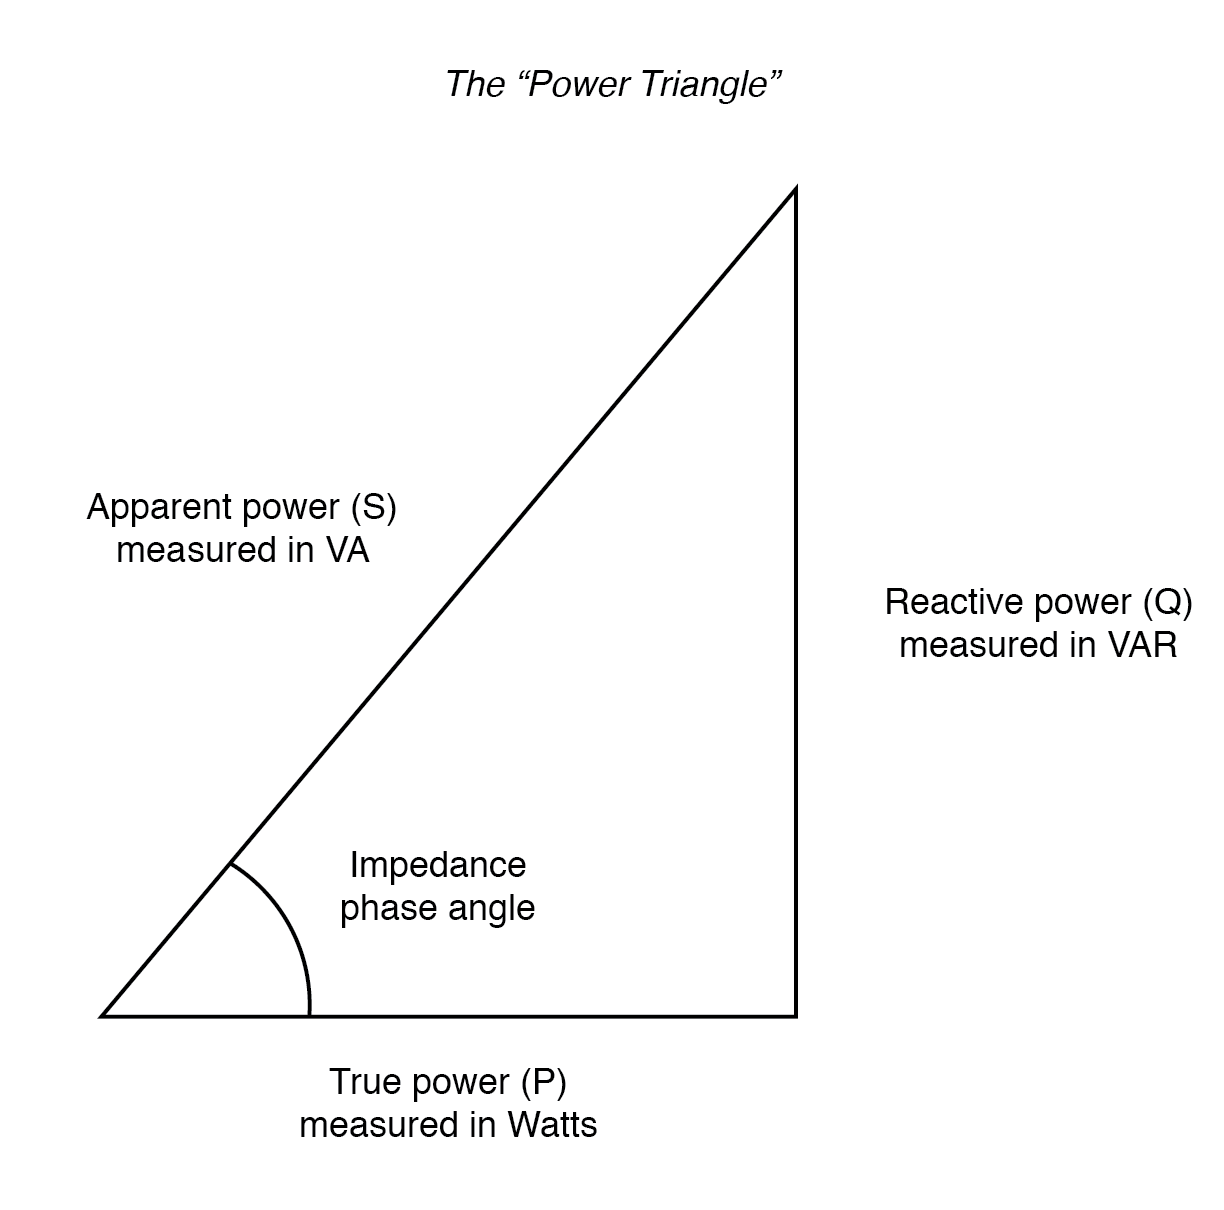
\includegraphics[scale=0.2]{figs/ch01/power_triangle.png}
\end{center}

\section{Impedance Matching}

\begin{pline}
    \item \textbf{Impedance:} the total resistance of a given electric component or AC circuit originating from reactive and resistance of the given system. Has both \textit{phase} and \textit{resistance} for AC. For DC, impedance has zero phase angle.
    \item \textbf{Impedance matching:} the process where the input impedance and the output impedance of a given electrical load are designed to reduce signal reflection and maximize the power transferred to the electric load.
\end{pline}

\subsection{Motivation}
Impedance matching has great use in high-frequency and high-speed devices. 

When designing applications of ultra-high frequencies, impedance matching becomes a difficult operation for designers. The challenge is also reflected while designing microwaves and radio frequency circuits. When you get a wrong impedance matching, expect distorted pulses and high signal reflections.

An increase in frequency decreases the window of errors. The electrical circuit works the best when we have a perfectly matched impedance. If the impedance matching is not done, expect the system to work abnormally because of the effects such as the signal reflections. The reflected waves cause data delays and distortion of the phase and minimize the ratio of signal to noise.

\begin{pline}
    \item Maximum power transfer occurs when the resistance of the voltage source is equal to the resistance of the load.
\end{pline}

We can show this by taking the derivative of the power function. At maximum power transfer, this derivative is equal to zero

\subsection{Examples}
\begin{enumerate}
    \item Suppose that we have a system that is modeled by the circuit below
        \begin{figure}[H]
    \centering
    \begin{circuitikz}[american]
        \draw (0,0)
        to[V, v=$V$, invert] (0,2)
        to[R, l=$R_{in}$, i=$i_{load}$] (2,2)
        to[R, l=$R_{load}$] (2,0)
        -- (0,0);
        \draw (2,2) -* (4,2) to[open, v=$V_{\text{out}}$] (4,0) -- (2,0);
    \end{circuitikz}    
\end{figure}
\begin{align*}
    P &= I_{load}^2 R_{load} = \frac{V^2 R_{load}}{(R_{in} + R_{load})^2} \\
    \frac{dP}{dR_{load}} &= \frac{V^2(R_{in} + R_{load})^2 - 2R_{load}(R_{in} + R_{load})V^2}{(R_{in} + R_{load})^4} \\
    &= 0 \Rightarrow R_{load} \\
    &= R_{in}
\end{align*}

    \item Suppose now you have the following circuit
        \begin{figure}[H]
    \centering
    \begin{circuitikz}
        \draw (0,0)
        to[C, l=$C$] ++(0,2)
        to[L, l=$L$] ++(3,0)
        to[R, l=$R$] ++(0,-2)
        to (0,0);
    \end{circuitikz}
\end{figure}

    \item \textbf{Transformer impedance matching:} set the turn ratio accordingly. Low voltage $\rightarrow$ fewer turns. 
        \begin{define}
            \[\text{Turns ratio }= \sqrt{\frac{\text{Source resistance}}{\text{Load resistance}}}\]
        \end{define}
    
    \item \textbf{Transmission line:} Transmission of electrical energy from the source to the load is done using a transmission line. While transferring this energy, it is important to zero or minimize energy losses that occur. For this to be possible, we should match the source and load impedances to the transmission line being used.
    
    The characteristic impedance is defined as the voltage and current wave ratio at any given point along the transmission line. 
    If the transmission line in discussion is long, then we expect to have a different characteristic impedance at different distances along this transmission line. 
    If we fail to do the impedance matching, the signs reaching the load will be reflected in the source of the origin, giving rise to a standing wave. 
    The amount of power reflected is measured using the coefficient of reflection, which is calculated using the equation below
        \begin{define}
            \[\Gamma  = \frac{Z_L - Z_0}{Z_L + Z_0}\]
            $Z_L$: line impedance, $Z_0$: characteristic impedance
        \end{define}

    \item Attenna and television
        \begin{center}
            \begin{circuitikz}
                \draw (0,0)
                to[sV, v<=$V_{in}$] ++(0,2)
                to[R, l=$R_A$] ++(3,0)
                to[R, l=$R_L$] ++(0,-2)
                to (0,0);
            \end{circuitikz}
        \end{center}
        $R_A$ is the resistance of the antenna is 150$\Omega$ and its cable while the TV's resistance is 600$\Omega$. Use the turns ratio formula to find the number of turns. Then set a transformer in between like in the image below.
        \begin{figure}[H]
            \centering
            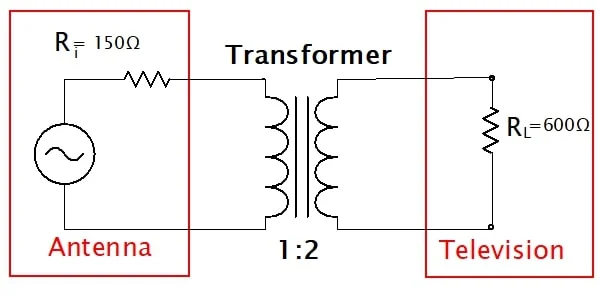
\includegraphics[scale=0.7]{figs/z_match_ex5.png}
        \end{figure}

    \item In the case of the headphone, the signal source is the device where the headphone is plugged. The headphone is the load. For the system to attain quality audio output, the source, and the load impedances must be matched. By matching the impedances, we make sure that there is maximum power transfer from the source of the audio to the headphone.

    When building portable devices, ensure that low-impedance headphones are built. This makes the system work well with proper sound quality.
\end{enumerate}

\section{Electrical Transformers}
Definitions for this section:
\begin{pline}
    
\end{pline}

\section{Sources}
\begin{enumerate}
    \item \href{https://www.youtube.com/watch?v=hRAyfJLZnC0&list=PLmK1EnKxphinxBub5hL0ZoJXWoqjkGE19}{katkimshow} Youtube Channel playlist "Introduction to Power Electronics (2023) for most of the introduction
    \item \href{https://www.youtube.com/watch?v=tClE8s6RZdg}{Why your Function Generator's output voltage reading can be wrong}
    \item \href{https://www.allaboutcircuits.com/textbook/alternating-current/chpt-11/true-reactive-and-apparent-power/}{True, Reactive, and Apparent Power}
    \item \href{https://www.analog.com/en/resources/glossary/impedance-matching.html}{impedance matching}
    \item \href{https://eepower.com/technical-articles/understanding-impedance-matching/#}{Understanding Impedance Matching}
    \item \href{https://eepower.com/power-electronics-textbook/vol-i-electrical-power-systems-design/chapter-5-impedance-matching-and-power-transfer/understanding-electrical-transformers/#}{Understanding Electrical Transformers}
\end{enumerate}